\documentclass{beamer}
\usepackage{beamerthemeshadow}
\usepackage[czech]{babel}
\usepackage[IL2]{fontenc}
\usepackage[utf8]{inputenc}
\usepackage{times}
\usepackage{hyperref}
\hypersetup{hidelinks}

\addtobeamertemplate{navigation symbols}{}{%
    \usebeamerfont{footline}%
    \usebeamercolor[fg]{footline}%
    \hspace{1em}%
    \insertframenumber/\inserttotalframenumber
}


\begin{document}

\title{Tým H*}  
\author{Hrabal Matěj\\
		Holop Patrik\\
		Halás Timotěj\\
		Hanák Jiří}
\date{\today} 

\frame{
\titlepage
} 



\section{Myšlenka} 
\frame{
\frametitle{Základní myšlenka}
\begin{columns}
\begin{column}{1\textwidth} 
\begin{figure}
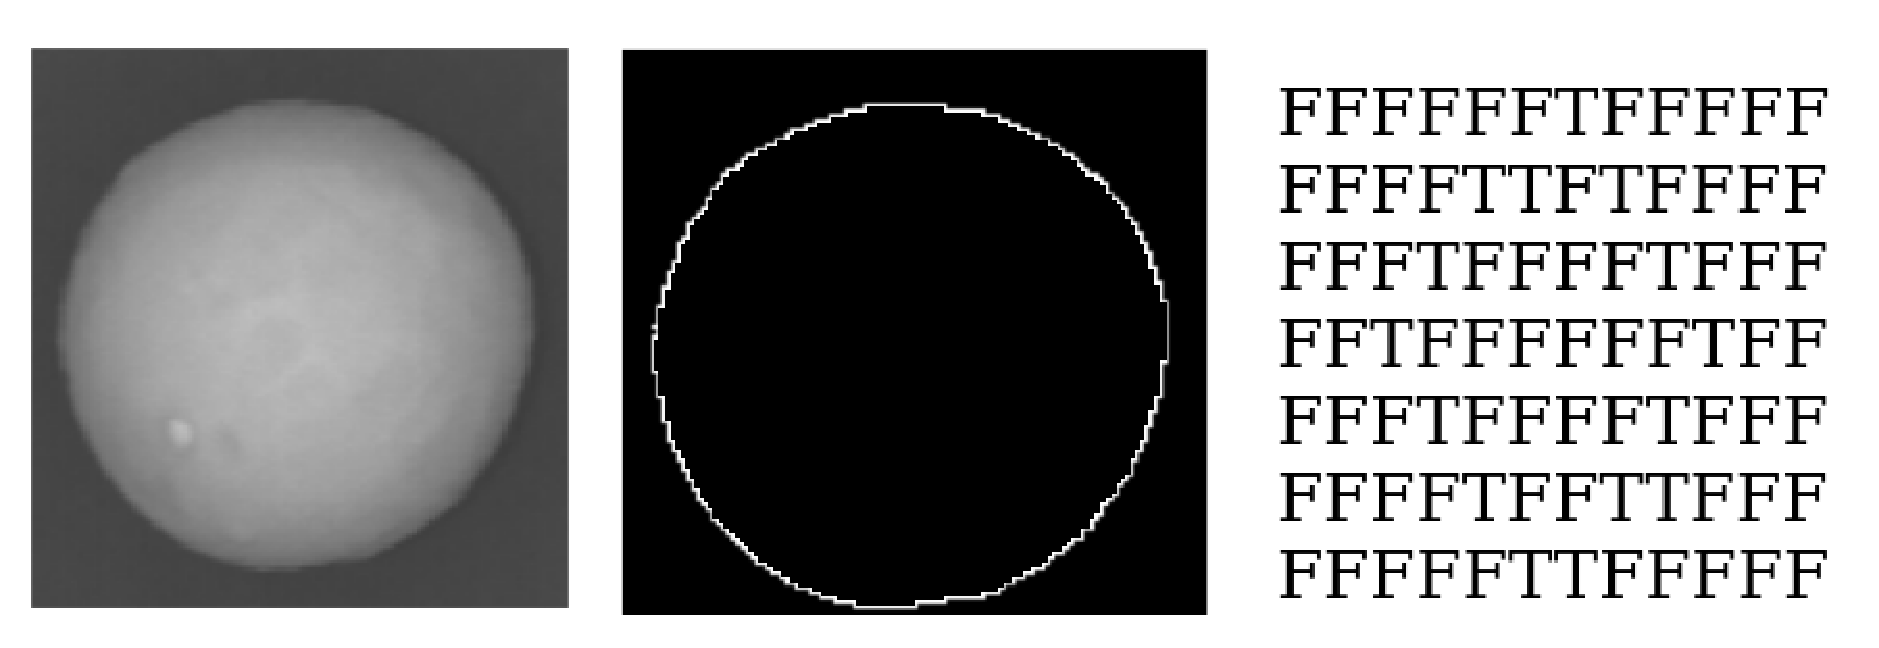
\includegraphics[scale=0.37]{principle} 
\end{figure}
\end{column}
\end{columns}
}

\frame{
\frametitle{Přístup}
Jazyk: Python

}


\section{Výsledky} 
\frame{
\frametitle{Naměřené výsledky}


}


\frame{
\frametitle{Konec}
\center{\Huge{Děkuji za pozornost}}
}
\end{document}
